\documentclass[../design_fonctionnement_sys.tex]{subfiles}
\begin{document}

\section{Fonctionnement du système}
Cette section portera sur des diagrammes qui présenteront le fonctionnement de différentes parties du système.

\subsection{Architecture de la communication client-serveur}
Le client communique avec le serveur via une collection de requêtes HTTP. Techniquement, nous utilisons la bibliotèque \texttt{CppRestSDK} pour envoyer des requêtes HTTP.

Pour vérifier qu'un joueur soit bien connecté, le joueur dispose d'un token d'authentification qui est envoyé avec chaque requête.
Ce token est généré lors de la connexion et est stocké dans le cache du client. Il n'est pas valide indéfiniment, et est régénéré à chaque nouvelle connexion.
Chaque requête est interceptée par le serveur, qui vérifie la validité du token. Si le token est valide, la requête est traitée, sinon, une erreur est renvoyée.
Ce token est envoyée pour toutes les requêtes qui nécessitent une authentification, comme par exemple, pour envoyer un message dans le chat, ou pour démarrer une partie.

De plus, bien que tout le code soit écrit en C++, nous avons décidé de nous inspiré des architectures REST utilisées dans les applications web.
C'est pour cela que nous avons décidé que toutes les requêtes seraient envoyées en format JSON, et les réponses sont également envoyées avec ce format.
Afin de pouvoir traiter le format JSON, nous utilisons la bibliotèque de Niels Lohmann, \href{https://github.com/nlohmann/json}{nlohmann/json}.

\subsection{Inscription}
Si le joueur possède déjà un compte, il a la possibilité de se connecter directement.
Le gestionnaire d'inscription (registerController) effectuera une première vérification des données saisies par l'utilisateur, 
notamment en s'assurant qu'aucun champ n'est laissé vide.

Une fois cette vérification effectuée, les données seront transmises au serveur via l'endpoint \texttt{api/register}. Ce dernier prendra comme argument la nom d'utilisateur et le mot de passe.

Ce dernier procédera ensuite à la vérification de la disponibilité du nom d'utilisateur. Afin de maximiser la sécurité, le mot de passe sera haché avant d'être stocké dans la base de données.
La base de donnée contiendra alors le nom d'utilisateur et le mot de passe haché. Cependant, pour une recherche dans la base de donnée, 
il est  bien plus efficace de donner un identifiant unique à chaque utilisateur. C'est pour cela que nous avons décidé de donner un identifiant unique à chaque utilisateur.
Ce dernier sera généré automatiquement lors de l'inscription et est récupérable via l'endpoint \texttt{api/login/uid}.

Maintenant que tout s'est bien déroulé, l'utilisateur va automatiquement être connecté. C'est à dire que le token d'authentification sera généré et envoyé au client.

\textit{Remarque:} Le token a deux fonctions: à savoir qui envoie le message, et savoir si la personne qui envoie le message est bien connecté.
Par exemple, le token est particulièrment utile pour le chat, car il permet de savoir qui envoie le message, et si l'utilisateur est bien connecté (pour éviter que tout le monde puisse récupérer les message d'un autre utilisateur).

\begin{figure}[H]
    \centering
    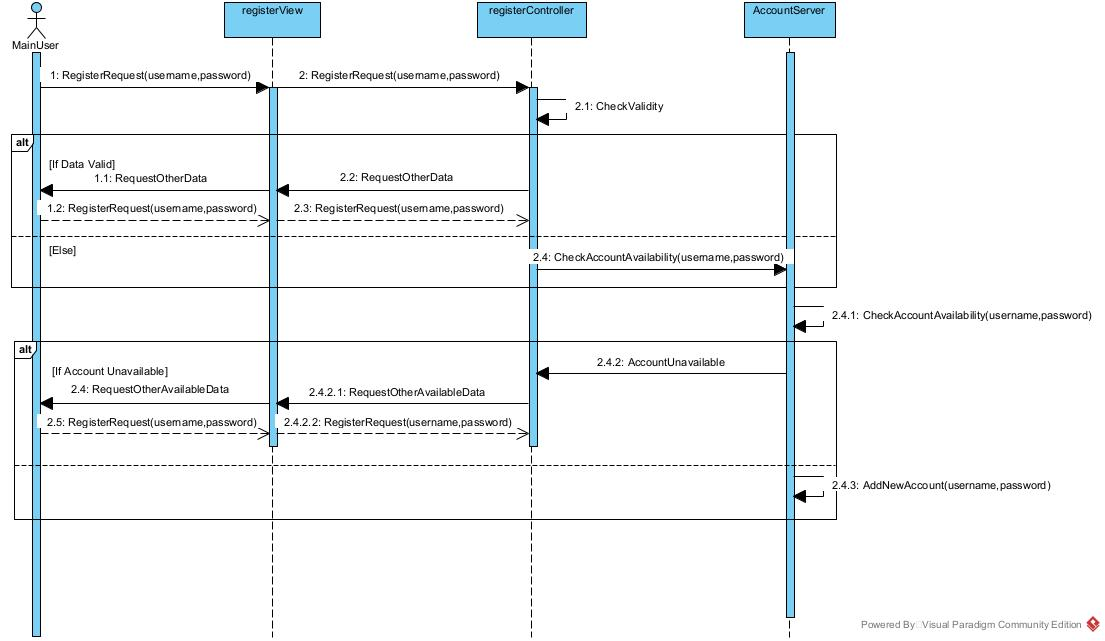
\includegraphics[scale=0.4]{img_design/RegisterSD.jpg}
    \label{fig:seq_match_client}
    \caption{Inscription}
\end{figure}
\newpage

\subsection{Connexion}
La connexion est en quelques sortes similaire à l'inscription. L'utilisateur doit saisir son nom d'utilisateur et son mot de passe, et le gestionnaire de compte va vérifier
si le compte est bien valide. Si c'est le cas, le serveur va générer un token d'authentification et l'envoyer au client. Dans le cas contraire,
le client va recevoir un code d'erreur.

\begin{figure}[H]
    \centering
    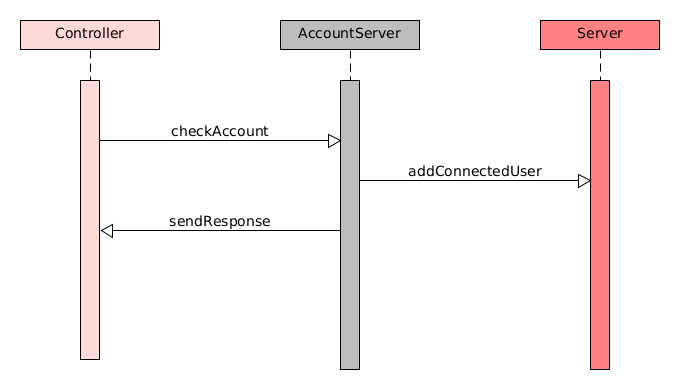
\includegraphics[scale=0.4]{img_design/connexion_seq.png}
    \label{fig:seq_match_client}
    \caption{Connexion}
\end{figure}


\subsection{Chat}
Le chat permet aux utilisateurs de communiquer les uns entre les autres. Il s'agit uniquement de \textit{whispers} (messages privés), qui ne comprennent que des messages textuels.
Le chat est complètement géré par le serveur, c'est-à-dire qu'aucun message n'est stocké par l'utilisateur.

L'utilisateur a alors simplement deux endpoint pour chatter: \texttt{api/chat/send} pour envoyer un message, et \texttt{api/chat/get} pour recevoir les messages.
Lors de chaque requête, l'utilisateur envoie son token et le nom de son ami. Le serveur vérifie alors si l'utilisateur est bien connecté, et si l'ami existe bien.
Si c'est le cas, le serveur peut alors effectuer toutes les manipulations nécessaires pour envoyer ou recevoir un message.

\begin{figure}[H]
    \centering
    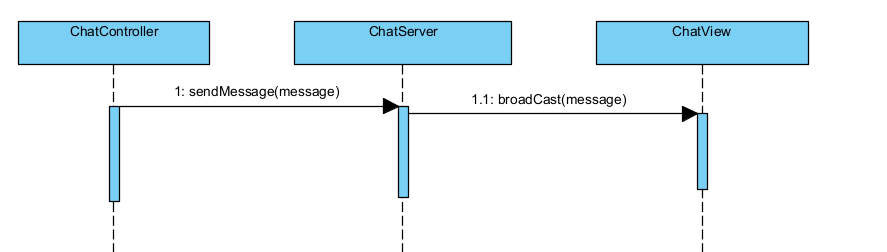
\includegraphics[scale=0.3]{img_design/Chat_DS.png}
    \label{fig:seq_match_client}
    \caption{Envoie d'un message}
\end{figure}

\subsection{Matchmaking}
Ce diagramme décrit la séquence d'actions réalisées lorsqu'un utilisateur veut créer/configurer une partie.

\begin{figure}[H]
    \centering
    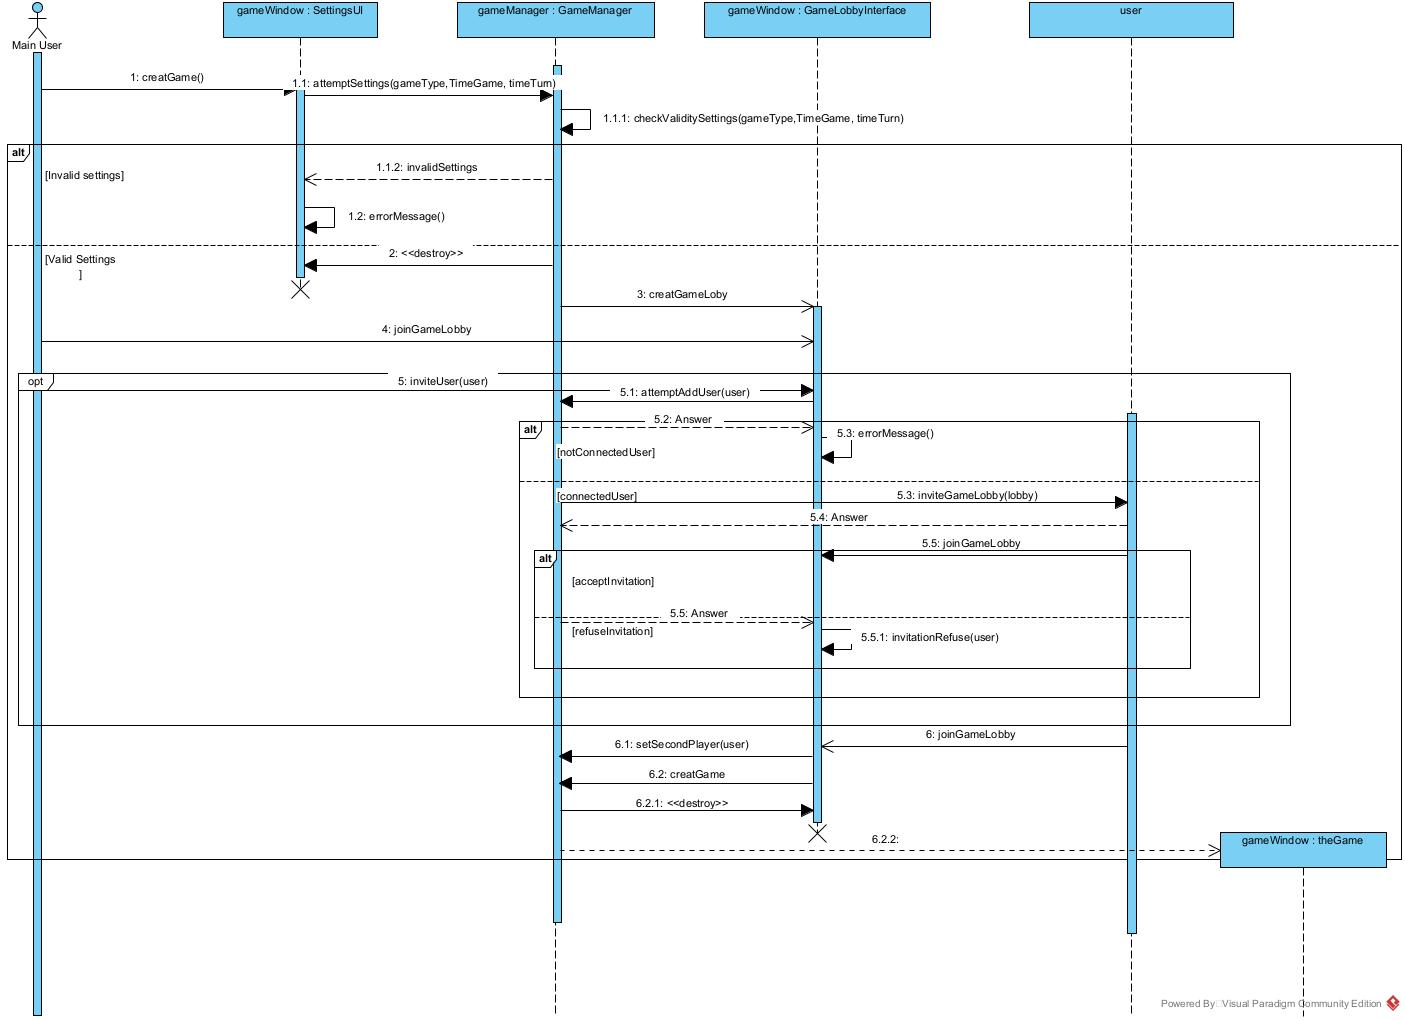
\includegraphics[scale=0.3]{img_design/PreLoby.jpg}
    \label{fig:seq_match_client}
    \caption{Matchmaking : Création du lobby}
\end{figure}

\newpage

\subsection{Lobby}
Ce diagramme décrit la séquence d'actions réalisés lorsqu'un utilisateur se trouve au stade de lobby et qu'il veut démarrer une partie.
Le deuxième joueur a déjà été fixé, et les bateaux doivent être placés sur le plateau pour que la partie puisse se lancer.
Mais avant de placer les bateaux, le plateau avec les deux boards est créé mais aussi 2 players. Un player est assigné à chaque user.

\begin{figure}[H]
    \centering
    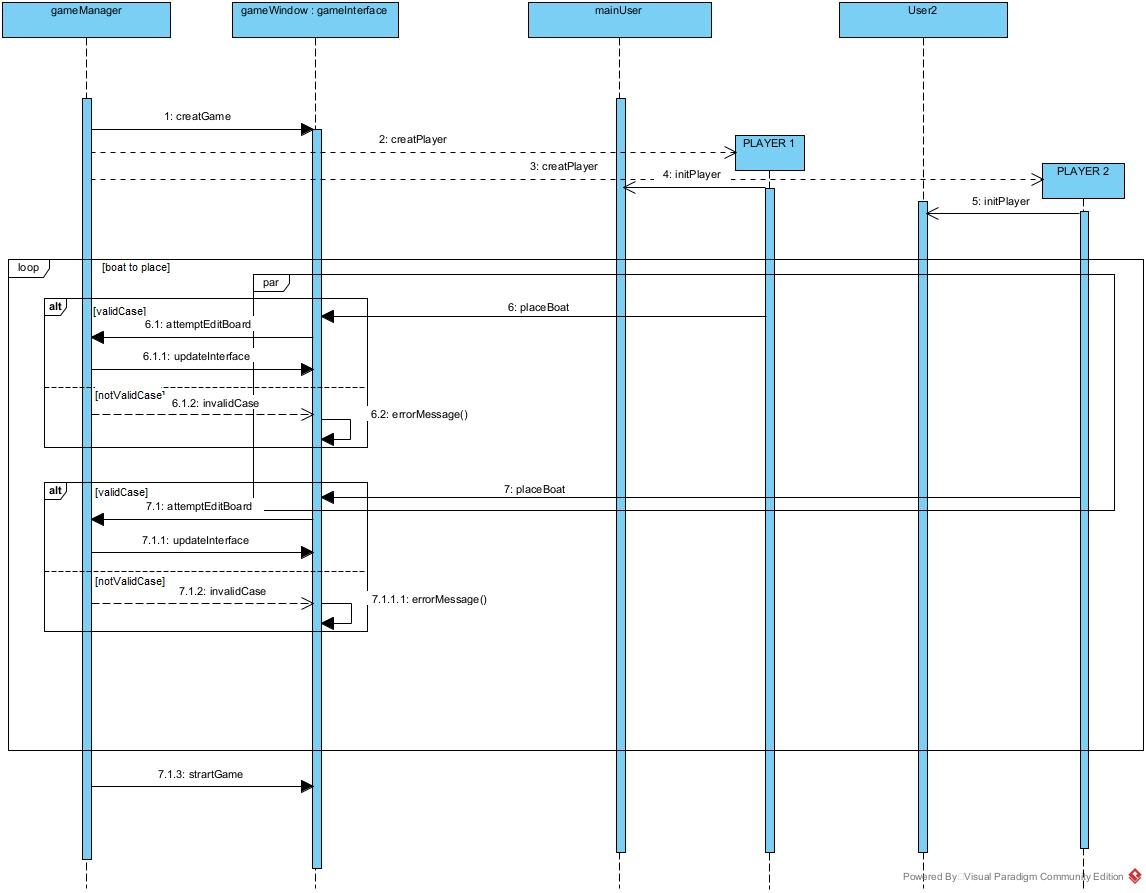
\includegraphics[scale=0.4]{img_design/PreGame.jpg}
    \label{fig:seq_match_server}
    \caption{Avant que la partie commence}
\end{figure}
\newpage

\subsection{Boucle de jeu}
La déroulement de la partie se passe au tour par tour. A tour de rôle le user transmet son action
mais l'action est gérée par player. Cela permet à une classe player d'avoir des points d'énergie, des actions et faire partie
d'une faction. L'action est d'abbord vérifiée pour savoir si la case ciblée est autorisée. Si c'est le cas le plateau
est modifié et l'interface est mise à jour.

Vu que nous utilisons une architecture RESTful pour la communication client-serveur, le client doit faire du polling pour savoir si c'est à son tour de jouer.
C'est à dire que le client doit envoyer une requête pour savoir si c'est à son tour de jouer. Si c'est le cas, le serveur renvoie une réponse positive, sinon, une réponse négative.

\begin{figure}[H]
    \centering
    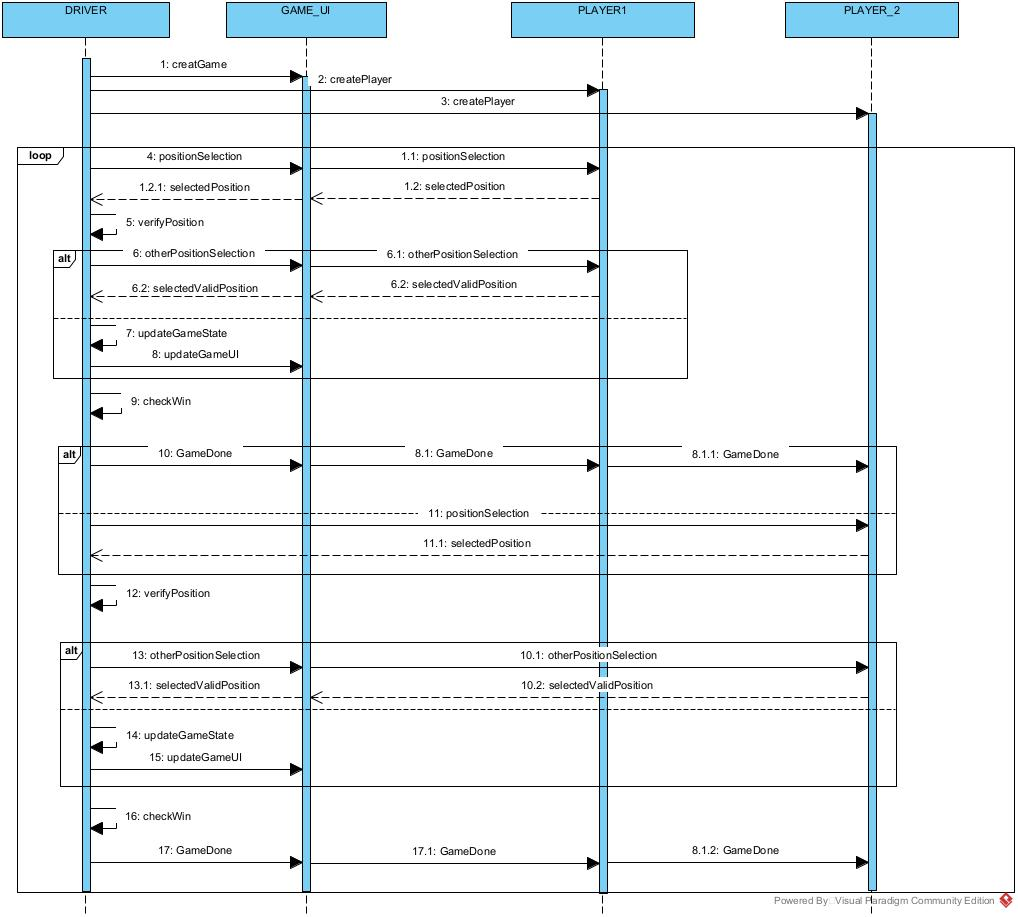
\includegraphics[scale=0.3]{img_design/Game.jpg}
    \label{fig:seq_gameloop_client}
    \caption{Boucle de jeu}
\end{figure}

\subsection{Gestion des comptes}
Afin de gérer tous les comptes utilisateur, leurs liste d'ami, et les messages privés, nous utilisons un moteur de base de donnée.
Cela nous permet de stocker toutes les informations de manière efficace. Dans notre cas, nous utilisons une base de donnée relationnelle, à savoir SQLite.
La plupart des informations qui sont fournies par le client sont stockées dans cette dernière.


\end{document}